\documentclass{beamer}[10]

\usepackage{graphicx}
\usepackage{xcolor}
\usepackage{tabto}
%\usepackage{beamerthemesplit}
\usepackage{tikz}
\usepackage{cancel}
\usepackage{verbatim}
\usepackage{fancybox}
\usepackage{enumerate}
\usepackage{amsmath,amssymb,amsthm,textcomp,mathtools}
\usepackage[super]{nth}
\usepackage[amssymb]{SIunits}
\usepackage{booktabs}
\usepackage{cancel}
\usepackage{bm}
\usepackage[utf8]{inputenc}
\usepackage{tabularx}
\usepackage{ragged2e}
\newcolumntype{Y}{ >{\RaggedRight\arraybackslash}X}
\usetikzlibrary{arrows,shapes}
\newcommand\T{\rule{0pt}{2.6ex}}
\newcommand\B{\rule[-1.2ex]{0pt}{0pt}}
\definecolor{UUcrimson}{RGB}{204,0,0}
\mode<presentation>
{ \usetheme{default}
  \usecolortheme[named=UUcrimson]{structure}
  \useinnertheme{circles}
  \setbeamercovered{transparent}
  \setbeamertemplate{blocks}[rounded]
  \usefonttheme[onlymath]{serif}
  \setbeamertemplate{navigation symbols}{}
  \setbeamertemplate{footline}[page number]
  \setbeamertemplate{navigation symbols}{}
  \setbeamercolor{section in toc}{fg=black,bg=white}
  \setbeamercolor{alerted text}{fg=UUcrimson!80!gray}
  \setbeamercolor*{palette primary}{fg=white,bg=UUcrimson}
  \setbeamercolor*{palette secondary}{fg=UUcrimson!70!black,bg=gray!15!white}
  \setbeamercolor*{palette tertiary}{bg=UUcrimson!80!black,fg=gray!10!white}
  \setbeamercolor*{palette quaternary}{fg=UUcrimson,bg=gray!5!white}
  \setbeamercolor*{palette sidebar primary}{fg=UUcrimson!10!black}
  \setbeamercolor*{palette sidebar secondary}{fg=white}
  \setbeamercolor*{palette sidebar tertiary}{fg=UUcrimson!50!black}
  \setbeamercolor*{palette sidebar quaternary}{fg=gray!10!white}
  \setbeamercolor{titlelike}{parent=palette primary,fg=white}
  \setbeamercolor{frametitle}{bg=UUcrimson}
  \setbeamercolor{frametitle right}{bg=UUcrimson}
  \setbeamercolor*{separation line}{}
  \setbeamercolor*{fine separation line}{}
}

\usetikzlibrary{backgrounds}
\makeatletter
\tikzstyle{every picture}+=[remember picture]
\tikzset{%
  fancy quotes/.style={
    text width=\fq@width pt,
    align=justify,
    inner sep=1em,
    anchor=north west,
    minimum width=\linewidth,
    font=\itshape
  },
  fancy quotes width/.initial={.8\linewidth},
  fancy quotes marks/.style={
    scale=8,
    text=white,
    inner sep=0pt,
  },
  fancy quotes opening/.style={
    fancy quotes marks,
  },
  fancy quotes closing/.style={
    fancy quotes marks,
  },
  fancy quotes background/.style={
    show background rectangle,
    inner frame xsep=0pt,
    background rectangle/.style={
      fill=gray!25,
      rounded corners,
    },
  }
}
\newenvironment{fancyquotes}[1][]{%
\noindent
\tikzpicture[fancy quotes background]
\node[fancy quotes opening,anchor=north west] (fq@ul) at (0,0) {``};
\tikz@scan@one@point\pgfutil@firstofone(fq@ul.east)
\pgfmathsetmacro{\fq@width}{\linewidth - 2*\pgf@x}
\node[fancy quotes,#1] (fq@txt) at (fq@ul.north west) \bgroup}
{\egroup;
\node[overlay,fancy quotes closing,anchor=east] at (fq@txt.south east) {''};
\endtikzpicture}
\makeatother

\usepackage{scalerel}[2014/03/10]
\usepackage{stackengine}
\usepackage{empheq}
\newcommand*\widefbox[1]{\fbox{\hspace{0.5em}#1\hspace{0.5em}}}

\newcommand\reallywidetilde[1]{\ThisStyle{%
  \setbox0=\hbox{$\SavedStyle#1$}%
  \stackengine{-.1\LMpt}{$\SavedStyle#1$}{%
    \stretchto{\scaleto{\SavedStyle\mkern.2mu\sim}{.5467\wd0}}{.4\ht0}%
%    .2mu is the kern imbalance when clipping white space
%    .5467++++ is \ht/[kerned \wd] aspect ratio for \sim glyph
  }{O}{c}{F}{T}{S}%
}}
\usepackage{media9}

\logo{
\includegraphics[width=0.75cm]{logo.jpg}}
\author[Gibbs]{Dr. Jeremy A. Gibbs}
\institute{Department of Mechanical Engineering\\University of Utah}
\date{Fall 2016}
\title{LES of Turbulent Flows: Lecture 4}
\begin{document}

%----------------------------------------------------------------------------------------
%	TITLE & TOC SLIDES
%----------------------------------------------------------------------------------------

\begin{frame} 
  \titlepage
\end{frame}

%------------------------------------------------

\begin{frame}
\frametitle{Overview}
\tableofcontents
\end{frame}

%------------------------------------------------
\section{One last review of turbulence (beat it into your heads)} %
%------------------------------------------------
\begin{frame}{Review: Properties of turbulent flows}

\begin{itemize}
	\item Unsteadiness: $u = f(\vec{x},t)$
	\item Three-dimensional: $\vec{x} = f(x_i)$ for any turbulent flow
	\item High vorticity: $\omega = \nabla \times \vec{u}$
	\item Mixing effect: turbulence acts to reduce gradients
	\item Continuous spectrum of scales: energy cascade described broadly by Kolmogorov's hypotheses
\end{itemize}

\end{frame}

%------------------------------------------------

\begin{frame}{Review: Kolmogorov's similarity hypothesis}
Kolmogorov's \nth{1} hypothesis
\begin{itemize}
	\item Smallests scales receive energy at a rate proportional to the dissipation of energy rate
	\item With this, he defined the Kolmogorov (dissipation) scales:\newline\newline
	length scale $$\eta = \left(\frac{\nu^3}{\epsilon}\right)^{\frac{1}{4}}$$
	time scale $$\tau = \left(\frac{\nu}{\epsilon}\right)^{\frac{1}{2}}$$
	velocity scale $$v = \frac{\eta}{\nu} = (\nu \epsilon)^{\frac{1}{4}}$$
\end{itemize}

\end{frame}

%------------------------------------------------

\begin{frame}{Review: Kolmogorov's similarity hypothesis}

\begin{itemize}
	\item Using these scales, we can define the ratios of the largest to smallest scales:\newline\newline
	length scale $$\frac{\ell_o}{\eta} \sim \text{Re}^{\frac{3}{4}}$$
	velocity scale $$\frac{U_0}{v} \sim \text{Re}^{\frac{1}{4}}$$
	time scale $$\frac{t_o}{\tau} \sim \text{Re}^{\frac{1}{2}}$$
\end{itemize}

\end{frame}

%------------------------------------------------

\begin{frame}{Review: Kolmogorov's similarity hypothesis}
Kolmogorov's \nth{2} hypothesis
\begin{itemize}
	\item In turbulent flow, a range of scales exists at very high Re where statistics of motion in a range $l$ ($\ell_o \gg \ell \gg \eta$) have a universal form that is determined only by $\epsilon$ (dissipation) and independent of $\nu$ (kinematic viscosity).
	\item Kolmogorov formed his hypothesis and examined it by looking at the PDF of velocity increments $\Delta u$.
\end{itemize}

\end{frame}

%------------------------------------------------

\begin{frame}{Review: Kolmogorov's similarity hypothesis}
\begin{itemize}
	\item We can examine this through $E(k)$, where $E(k)dk =$TKE contained between $k$ and $k+dk$.
	\item What are the implications of Kolmogorov’s hypothesis for $E(k)$? -- K41$\Rightarrow E(k) = f(k,\epsilon)$
	\item By dimensional analysis, Kolmogorov showed: $$E(K) = c_k \epsilon^{2/3}k^{-5/3}$$ Kolmogorov's -5/3 power law.
\end{itemize}

\end{frame}

%------------------------------------------------
\begin{frame}{Review: Kolmogorov's similarity hypothesis}

Example energy spectrum
\begin{figure}
	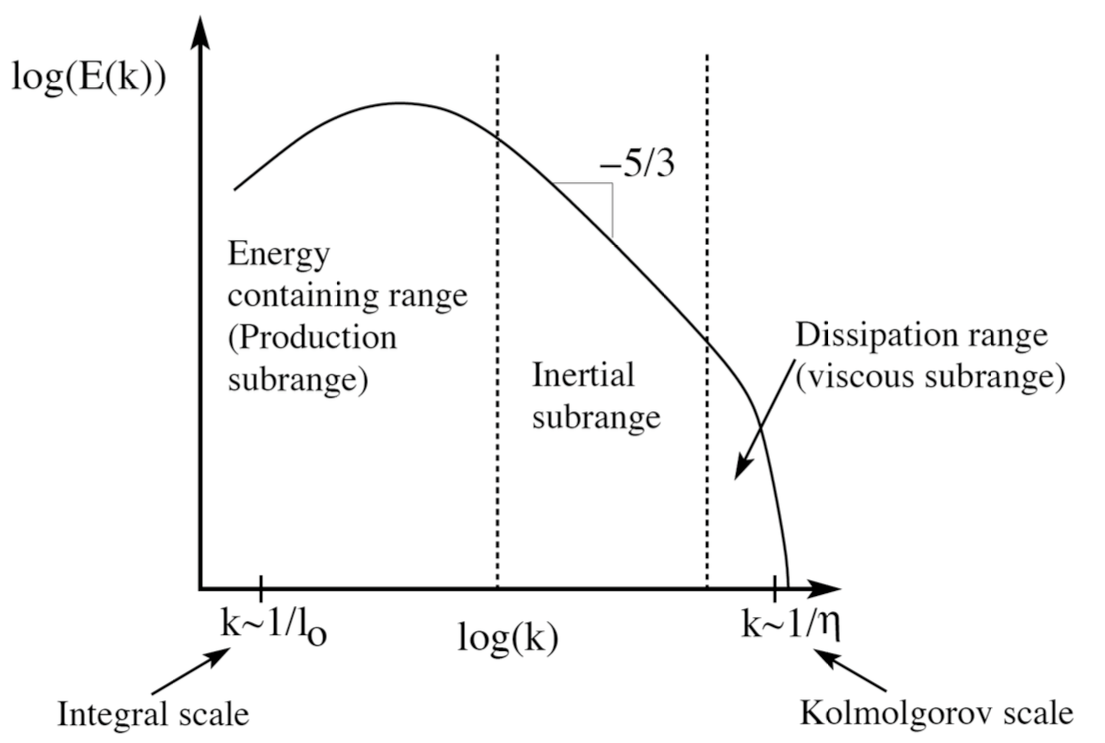
\includegraphics[width=\textwidth]{spectrum2.png}
\end{figure}
\end{frame}

%------------------------------------------------
\section{Numerical simulations} %
%------------------------------------------------
\begin{frame}{Degrees of freedom and numerical simulations}

\begin{itemize}
	\item We now have a description of turbulence and the range of energy containing scales (the dynamic range) in turbulence.
	\item In computational fluid dynamics (CFD), we need to discretize the equations of motion using either difference approximations (finite differences) or as a finite number of basis functions (e.g., Fourier transforms).
	\item Essentially, a continuous solution is approximated by a finite set of values corresponding as closely as possible with the values of the solution on a grid of discrete positions in space.
\end{itemize}
\end{frame}

%------------------------------------------------

\begin{frame}{Degrees of freedom and numerical simulations}

\begin{itemize}
	\item To capture all of the dynamics (degrees of freedom) in a turbulent flow, we must consider the required amount of discrete values needed for an accurate approximation.
	\item We need a grid fine enough to capture the smallest \textit{and} the largest scales of motion ($\eta$ and $\ell_o$).
\end{itemize}
\end{frame}

%------------------------------------------------

\begin{frame}{Degrees of freedom and numerical simulations}

\begin{itemize}
	\item From K41, we know that $\ell_o/\eta\sim \text{Re}^{3/4}$ and there exists a continuous range of scales between $\eta$ and $\ell_o$.
	\item We will assume that we need $n$ grid points per increment $\eta$. Note that $n$ can vary, but a value of 3 to 5 is often suggested.
	\item Thus, in each direction, the number of required grid points is
	$$N_i = \frac{\ell_o}{(\eta/n)} = n\ \frac{\ell_o}{\eta} \sim n\ \text{Re}^{3/4}$$
	\item Remember that turbulence is 3D, so the total number of grid points needed to accurately estimate the flow is
	$$N = \left(n\ \text{Re}^{3/4} \right)^3 = \boxed{n^3\ \text{Re}^{9/4}}$$
\end{itemize}
\end{frame}


%------------------------------------------------

\begin{frame}{Degrees of freedom and numerical simulations}

\begin{itemize}
	\item Let's revisit our example of a typical atmospheric boundary layer flow:$$U_o\sim10\ \metre\ \reciprocal\second,\ \ell_o\sim10^3\ \metre,\ \nu \sim 10^{-5}\ \square\metre\ \reciprocal\second$$
	which gives us, $$\text{Re} = \frac{U_o \ell_o}{\nu} \sim \frac{(10\ \metre\ \reciprocal\second)(10^3\ \metre)}{10^{-5}\ \square\metre\ \reciprocal\second} \sim 10^9$$
	\item thus, the number of grid points required to fully resolve this flow (assuming $n$ = 3) is
	$$N = 9 \times (10^9)^{9/4}\sim 1.6\times 10^{21} \text{!!!!!!!}$$
	Note: current capabilities of modern computing allow for grid sizes with $\mathcal{O}(10^{11})$ points.
\end{itemize}
\end{frame}

%------------------------------------------------

\begin{frame}{Degrees of freedom and numerical simulations}

\begin{itemize}
	\item What does a simulation of a typical atmospheric boundary layer flow using a grid with $1.6\times 10^{21}$ points buy? (recall $\eta \sim 0.18\ \milli\meter$)
	$$\l_i = \eta * \left(1.6\times 10^{21}\right)^{1/3} \sim 2\ \kilo\metre$$
	This means we can simulate a $2\ \kilo\metre \times 2\ \kilo\metre \times 2\ \kilo\metre$ cube.
	Think how big the atmosphere is and then be depressed.
\end{itemize}
\end{frame}

%------------------------------------------------

\begin{frame}{Degrees of freedom and numerical simulations}

\begin{itemize}
	\item When will we be able to directly simulate all the scales of motion in a turbulent flow?
	\item A couple of studies used historical data from the literature to build a model that predicts this question (see Voller and Port\'{e}-Agel, 2002 and Bou-Zeid, 2014 handouts).
	\item VP02 derived a model based on Moore's Law $$P = A\ 2^{0.6667\text{Y}}$$ where $A$ is the computer power at reference year Y=0.
\end{itemize}
\end{frame}

%------------------------------------------------

\begin{frame}{Degrees of freedom and numerical simulations}

\begin{itemize}
	\item VP02 used a reference year of 1980 and used $A=100$ and $A=10,000$.
	\item The best fit was $$N(t) = 691 \times 2^{0.697(\text year - 1980)}$$
	\begin{figure}
		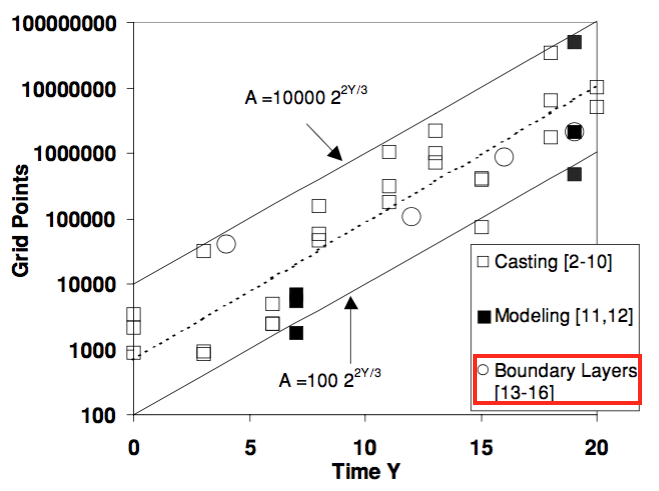
\includegraphics[width=0.7\textwidth]{mooreslaw1.png}
	\end{figure}
\end{itemize}
\end{frame}

%------------------------------------------------

\begin{frame}{Degrees of freedom and numerical simulations}
	\begin{figure}
		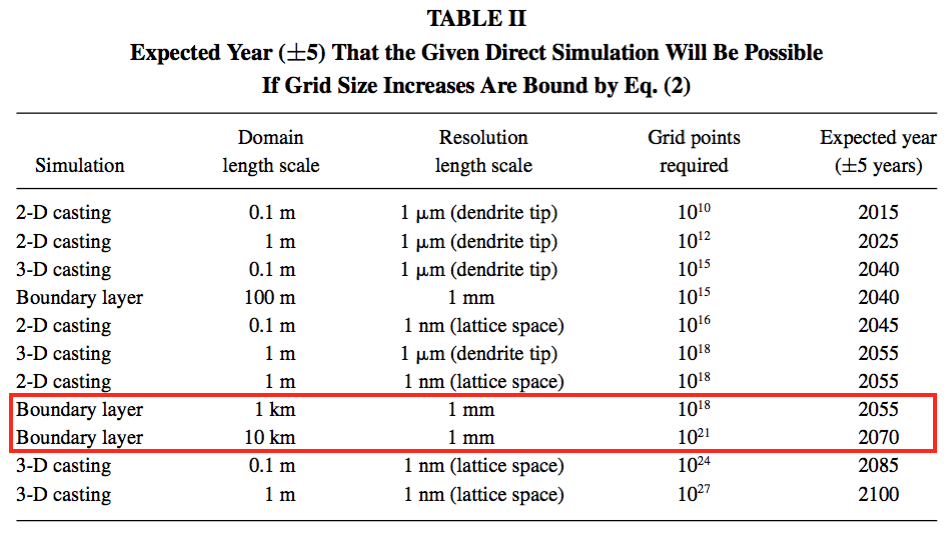
\includegraphics[width=1\textwidth]{mooreslaw2.png}
	\end{figure}
\end{frame}

%------------------------------------------------

\begin{frame}{Degrees of freedom and numerical simulations}

\begin{itemize}
	\item BZ14 updated VP02 using data between 2002 and 2014. It turns out that VP02 was too optimistic. Be more depressed.
	\begin{figure}
		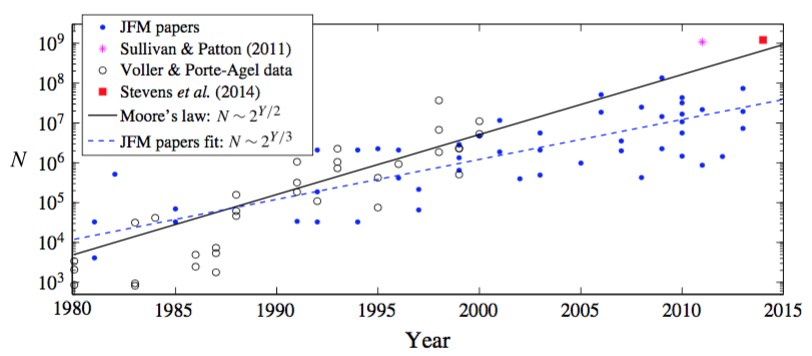
\includegraphics[width=0.9\textwidth]{mooreslaw3.png}
	\end{figure}
\end{itemize}
\end{frame}

%------------------------------------------------

\begin{frame}{Degrees of freedom and numerical simulations}

\begin{itemize}
	\item The Re of relevant flows are orders of magnitude too large for current computational resources.
	\item Thus, DNS will not be a suitable tool for a long time (relevant to our brief time on Earth).
	\item The only alternative is to simplify the description of a flow and try to model the small scales instead of resolving them.
	\item This makes the problem less demanding computationally, but harder in many aspects due to the modeling requirement.
	\item Before we delve into methods that accomplish this reduction of complexity, we need to understand how we describe a flow.
\end{itemize}
\end{frame}

%------------------------------------------------
\section{Equations of motion} %
%------------------------------------------------
\begin{frame}{Equations of motion}

\begin{itemize}
	\item Turbulent flow (and fluid dynamics in general) can be mathematically described by the Navier-Stokes equations (see Bachelor, 1967 for a derivation, see also Pope chapter 2).
	\item The primary goal of CFD (and LES) is to solve the discretized equations of motion.
	\item We use the continuum hypothesis (\textit{i.e.}, $\eta \gg$ mean free path of molecules) so that $$u_i = u_i(x_j,t) \qquad \text{and} \qquad \rho = \rho(x_j,t)$$
\end{itemize}
\end{frame}

%------------------------------------------------
\begin{frame}{Equations of motion: conservation of mass}

\begin{itemize}
	\item Conservation of mass $$\left.\frac{dm}{dt}\right|_{sys} = 0$$
	\item We can use Reynolds Transport Theorem (RTT, see any fluids book)
	$$\left.\frac{dm}{dt}\right|_{sys} = \frac{\partial}{\partial t} \underbrace{\int_{CV} \rho dV}_{\text{rate of increase in CV}} + \underbrace{\int_{CS} \rho \vec{V} \cdot d\vec{A}}_{\text{net flux leaving CV}} = 0$$
	Another way of saying that:\newline Production + Input = Change (in time) + Output (PICO).
\end{itemize}
\end{frame}

%------------------------------------------------
\begin{frame}{Equations of motion: conservation of mass}

\begin{itemize}
	\item We can use Gauss's theorem and shrink the control volume to an infinitesimal size:
	$$\frac{\partial \rho}{\partial t} + \frac{\partial}{\partial x_i}(\rho u_i) = 0$$
	This is the differential form of the conservation of mass.
\end{itemize}
\end{frame}

%------------------------------------------------
\begin{frame}{Equations of motion: conservation of momentum}

\begin{itemize}
	\item Conservation of momentum (Newton's \nth{2} law)
	$$ \sum \vec{F} = \left.\frac{d(m\vec{V})}{dt}\right|_{sys}$$
	We can again apply RTT and Gauss's theorem
	$$\frac{\partial(\rho u_i)}{\partial t} + \frac{\partial (\rho u_i \rho u_j)}{\partial x_j} = \frac{\partial }{\partial x_j} \left( 2\mu S_{ij} - \frac{2}{3} \mu \delta_{ij} \frac{\partial u_i}{\partial x_i}\right) - \frac{\partial P}{\partial x_i} + \rho g_i$$
	where $$S_{ij} = \frac{1}{2}\left( \frac{\partial u_i}{\partial x_j} + \frac{\partial u_j}{\partial x_i} \right)$$ is the rate of strain (deformation) tensor.\newline\newline
	This is the differential form of the conservation of momentum.
	\end{itemize}
\end{frame}

%------------------------------------------------
\begin{frame}{Equations of motion: conservation of energy}

\begin{itemize}
	\item Conservation of energy (\nth{1} law of thermodynamics)
	$$\dot Q - \dot W = \left.\frac{dE}{dt}\right|_{sys}$$
	If we use $e = c_v T$ (specific internal energy and $q_i = -K \partial T/\partial x_i$ (where $c_v$ is the specific heat, $T$ is temperature, and $q_i$ is the thermal flux), then we arrive at
	\begin{align*}
	\frac{\partial(\rho E)}{\partial t} &+ \frac{\partial}{\partial x_i} \left[u_i(P+E)\right] = \\&\rho \dot q + \frac{\partial q_i}{\partial x_i} + \frac{\partial}{\partial x_i} \left[ u_j \left( 2\mu S_{ij} - \frac{2}{3} \mu \delta_{ij} \frac{\partial u_i}{\partial x_i}\right)\right]
	\end{align*}
	This is the differential form of the conservation of energy.
\end{itemize}
\end{frame}

%------------------------------------------------
\begin{frame}{Equations of motion: incompressible flow}

Let's consider incompressible flow (\textit{i.e.}, the density of a fluid element does not change during its motion)
\begin{itemize}
	\item Conservation of mass $$\frac{\partial u_i}{\partial xi} = 0$$
	 \textit{i.e.}, divergence of the flow velocity is zero.
	\item Conservation of momentum $$\frac{\partial u_i}{\partial t} + \frac{\partial u_i u_j}{\partial x_j} = -\frac{1}{\rho} \frac{\partial P}{\partial x_i} + \nu \frac{\partial^2 u_i}{\partial x_j^2} + F_i$$
\end{itemize}
\end{frame}

%------------------------------------------------
\begin{frame}{Equations of motion: incompressible flow}

Let's consider incompressible flow (\textit{i.e.}, the density of a fluid element does not change during its motion)
\begin{itemize}
	\item Conservation of scalar (temperature, species, etc)$$\frac{\partial \theta}{\partial t} + \frac{\partial u_i \theta}{\partial x_j} = \nu_{\theta}\frac{\partial^2 \theta}{\partial x_j^2} + Q$$
	where $$\nu_{\theta} = \frac{\nu}{\text{Sc}} = \frac{\nu}{\text{Pr}}$$
	and Sc is the Schmidt number (used for scalars) and Pr is the Prandtl number (used for temperature).
\end{itemize}
\end{frame}

%------------------------------------------------
\begin{frame}{Equations of motion: incompressible flow}

\begin{itemize}
	\item Recall that
	$$\text{Sc} = \frac{\nu}{D} = \frac{\text{viscous diffusion rate}}{\text{molecular diffusion rate}}$$
	and $$\text{Pr} = \frac{\nu}{\alpha} = \frac{\text{viscous diffusion rate}}{\text{thermal diffusion rate}}$$
\end{itemize}
\end{frame}

%------------------------------------------------
\begin{frame}{Equations of motion: non-dimensional}

\begin{itemize}
	\item We can non-dimensionalize these equations by using a velocity scale ($U_o$) and length ($\ell_o$) scale. For example, the free-stream velocity and the boundary layer depth.
	\item Conservation of mass $$\frac{\partial u_i^*}{\partial x_i^*} = 0$$
	\item Conservation of momentum: $$\frac{\partial u_i^*}{\partial t*} + \frac{\partial u_i^* u_j^*}{\partial x_j^*} = -\frac{\partial P^*}{\partial x_i^*} + \frac{1}{\text{Re}} \frac{\partial^2 u_i^*}{\partial {x^*_j}^2} + F_i^*$$
	where Re is based on our velocity and length scales.
\end{itemize}
\end{frame}

%------------------------------------------------
\begin{frame}{Equations of motion: non-dimensional}

\begin{itemize}
	\item For any general scalar
	$$\frac{\partial \theta^*}{\partial t^*} + \frac{\partial u_i^* \theta^*}{\partial x_j^*} = \frac{1}{\text{Sc Re}} \frac{\partial^2 \theta^*}{\partial {x_j^*}^2} + Q^*$$
	generally, Sc $\sim 1$ and Pr $\sim 0.72$ (for air).
\end{itemize}
\end{frame}

%------------------------------------------------
\begin{frame}{Properties of Navier-Stokes equations}

\begin{itemize}
	\item \underline{Reynolds number similarity} - for a range of Re, the equations of motion can be considered invariant to transformations of scale. 
	\item \underline{Time and space invariance} - The equations are invariant to shifts in time or space, \textit{i.e.}, we can define the shifted space variable $$\hat x = \bar x/L, \text{where } \bar x = x - X$$
	\item \underline{Rotational and reflection invariance} -  The equations are invariant to rotations and reflections about a fixed axis. 
	\item \underline{Invariance to time reflections} - The equations are invariant to reflections in time. They are the same going backward or forward in time.
	\item \underline{Galilean invariance} - The equations are invariant to constant velocity translations
	$$\hat x = x - Vt$$
\end{itemize}
\end{frame}
%------------------------------------------------
\begin{frame}{Reynolds number similarity}

\begin{itemize}
	\item As an example of using Reynolds number similarity to make DNS available.
	\item Recall our example of atmospheric scales that gave a Re of $10^9$? We cannot afford this, but if we change the viscosity $\nu$ from $10^{-5}$ to 1, then Re = $10^4$ - which is doable.
	\item In fact, all dimensional scales match those of a typical laboratory experiment.
	\item We can use Reynolds number similarity to apply findings of our flow using the modified Re to that of a typical atmosphere.
\end{itemize}
\end{frame}

%------------------------------------------------
\begin{frame}{Reynolds number similarity}

\begin{figure}
	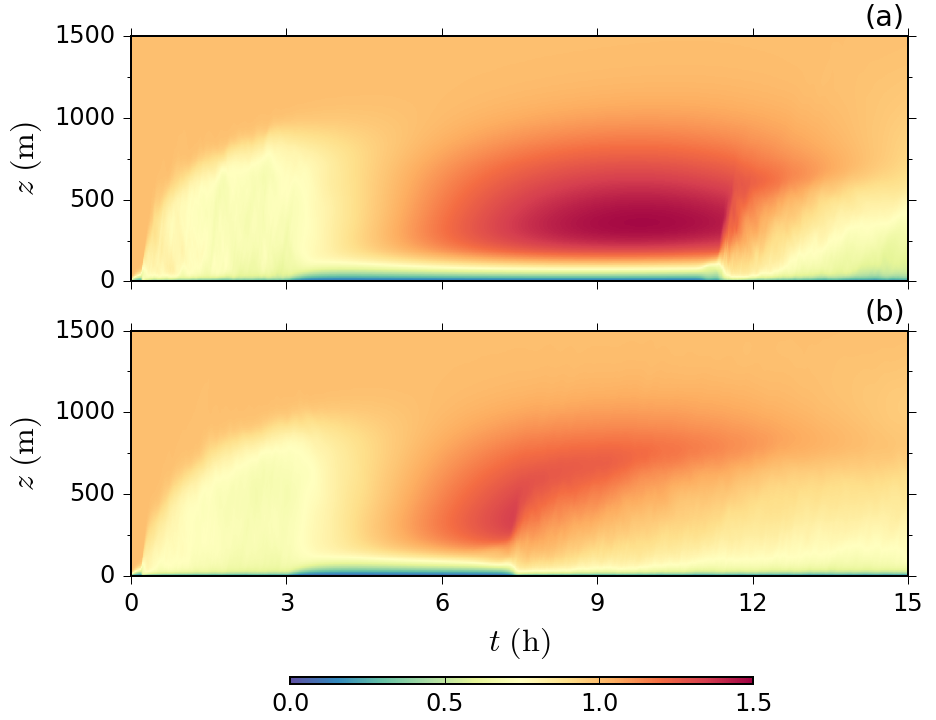
\includegraphics[width=0.8\textwidth]{jet1}
	\caption{Velocity from DNS of a low-level jet. (a) and (b) have different slope angles.}
\end{figure}
\end{frame}

%------------------------------------------------
\begin{frame}{Reynolds number similarity}

\begin{figure}
	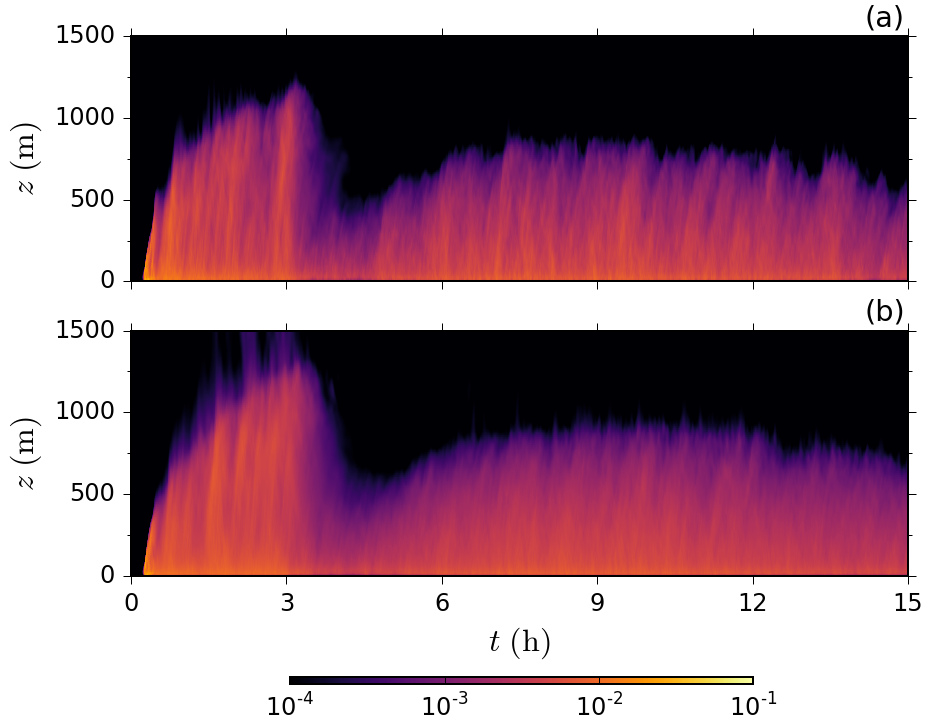
\includegraphics[width=0.8\textwidth]{jet2}
	\caption{TKE from DNS of a low-level jet. (a) and (b) have different slope angles.}
\end{figure}
\end{frame}

%------------------------------------------------
\begin{frame}{Reynolds number similarity}
\begin{itemize}
	\item You see that by changing the scaling, we still get results that seem to match the behavior of a flow with a larger Re.
	\item This is an example of using Reynolds number similarity.
\end{itemize}
\end{frame}


%------------------------------------------------






















%------------------------------------------------

\end{document}

